\documentclass[18pt]{beamer}

\usepackage[utf8]{inputenc}
\usepackage{default}
\usepackage{graphicx}
\usepackage{amsmath}
\usepackage{amsthm}
\usepackage{amsfonts}
\usepackage{amssymb}
\usepackage{tikz}
\usetikzlibrary{tikzmark,decorations.pathreplacing}
\usefonttheme{professionalfonts}

\usetheme{Warsaw}

\beamertemplatenavigationsymbolsempty
\addtobeamertemplate{navigation symbols}{}{%
    \usebeamerfont{footline}%
    \usebeamercolor[fg]{footline}%
    \hspace{1em}%
    \insertframenumber/\inserttotalframenumber
}

\useoutertheme{smoothbars}
\useinnertheme[shadow=true]{rounded}
\usecolortheme{whale}



%\newtheorem{definition}{Definition}
\begin{document}

\title{Formalisation of the Delaunay triangulation}
\author{Clément Sartori\\ Under the supervision of Yves Bertot}
\begin{frame}
 \maketitle
 \end{frame}
% \begin{frame}
%  \tableofcontents
% \end{frame}

\section{Introduction}

\begin{frame}
 Goals of the internship:
 \begin{enumerate}
  \item<1-> Formalise the Delaunay triangulations.
  \item<2-> Study some of the processes involved in constructing a Delaunay triangulation.
 \end{enumerate}
\begin{overprint}
\onslide<3->
 What I did:
 \begin{itemize}
 \item<4-> Formalise in Coq the abstract concept of Delaunay triangulations.
 \item<5-> Prove some useful hypotheses and geometric lemmas.
 \item<6-> Write two operations that are part of an algorithm to compute Delaunay triangulations and prove their correctness.
 \item<7-> Write an instantiation of the abtrast concept, with implementations for the functions.
 \end{itemize}
\end{overprint}

\end{frame}

\subsection{Triangulations}
\begin{frame}{Applications}
 Delaunay triangulations have lots of applications:
 \begin{itemize}
  \item<1,2,3,4> Shape morphing.
  \item<2,3,4> Modelise cellular coverage maps.
  \item<3,4> Path planning.
 \end{itemize}
\onslide<4>

Use of Delaunay triangulations algorithms in mission-critical software for autonomous vehicles.

 \vspace{0.3cm}
 
Continuation of a previous work by Yves Bertot and Jean-Francois Dufourd, in a more abstract way.

\end{frame}

\begin{frame}{Definition}

 A triangulation $T$ of a subset $X$ of $\mathbb{R}^d$ is a tiling of this subset with simplices such
that:
\begin{itemize}
 \item<1-> the intersection of two distinct simplices is either empty or a common face of these simplices;
 \item<2-> every bounded set of $\mathbb{R}^d$ cuts a finite number of simplices of $T$;
 \item<3-> the union of the simplices of T is X itself.
\end{itemize}

\begin{overprint}
\onslide<3>
\begin{figure}
  \centering
  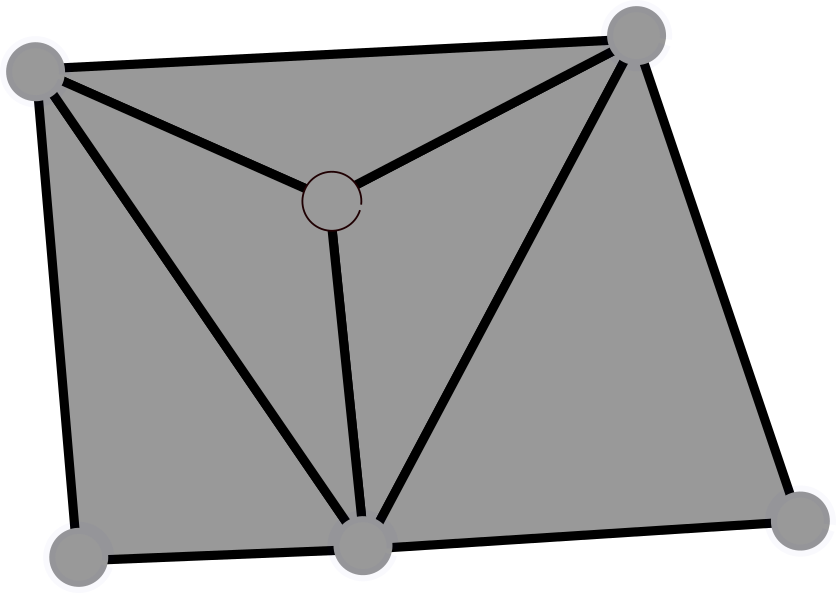
\includegraphics[scale=1.5]{Trig1}
  \caption{\label{Trig1} This is a triangulation of the convex hull of the points.}
\end{figure}

\onslide<4>
\begin{figure}
  \centering
  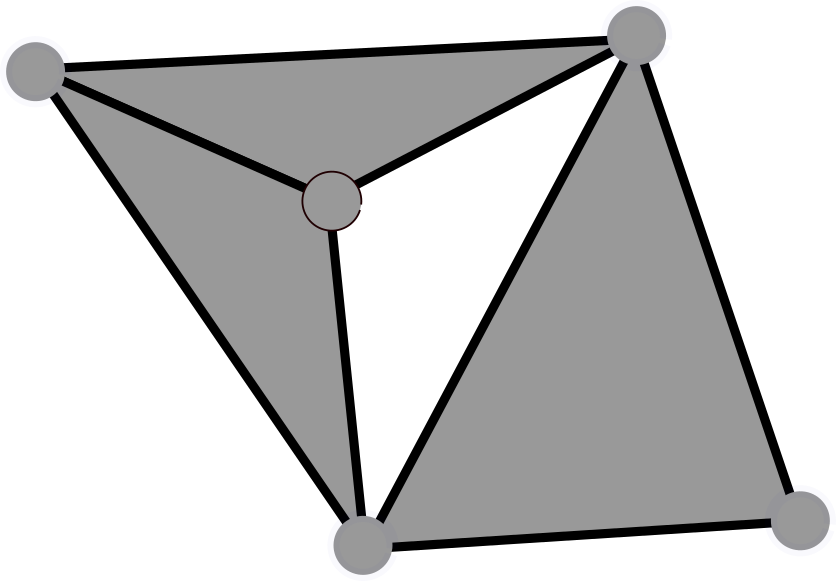
\includegraphics[scale=1.5]{NotTrig1}
  \caption{\label{NotTrig1} This is not a triangulation of the convex hull of the points.}
\end{figure}

\onslide<5>
\begin{figure}
  \centering
  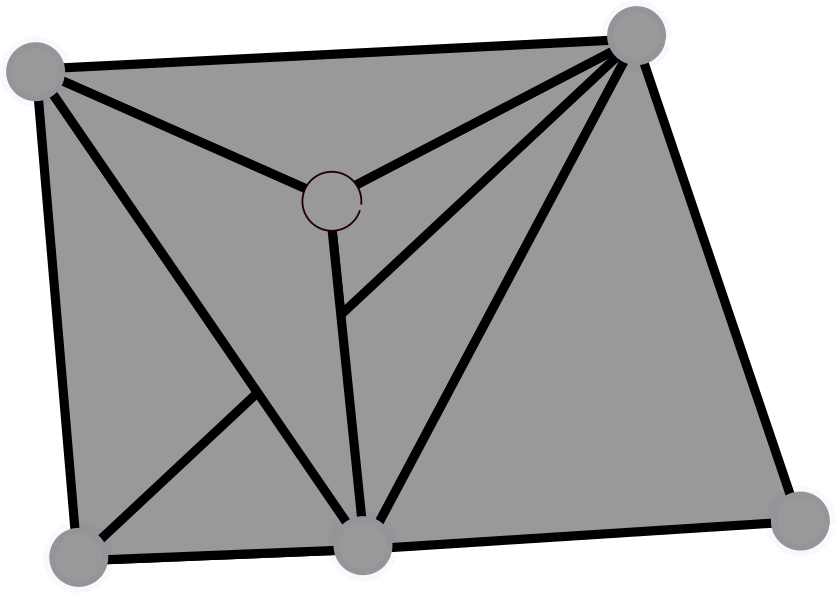
\includegraphics[scale=1.5]{NotTrig2}
  \caption{\label{NotTrig1} This is not a triangulation of the convex hull of the points.}
\end{figure}
\end{overprint}
\end{frame}

\begin{frame}{Delaunay triangulations}
 
 \begin{definition}
  A triangulation $T$ of the convex hull of a set of points $D$ is said to be a Delaunay triangulation if no point of $D$ is in the circumcircle of a triangle of T.
 \end{definition}
Intuitively, a Delaunay triangulation maximises the smallest angle of every triangles.
 \begin{figure}
\centering
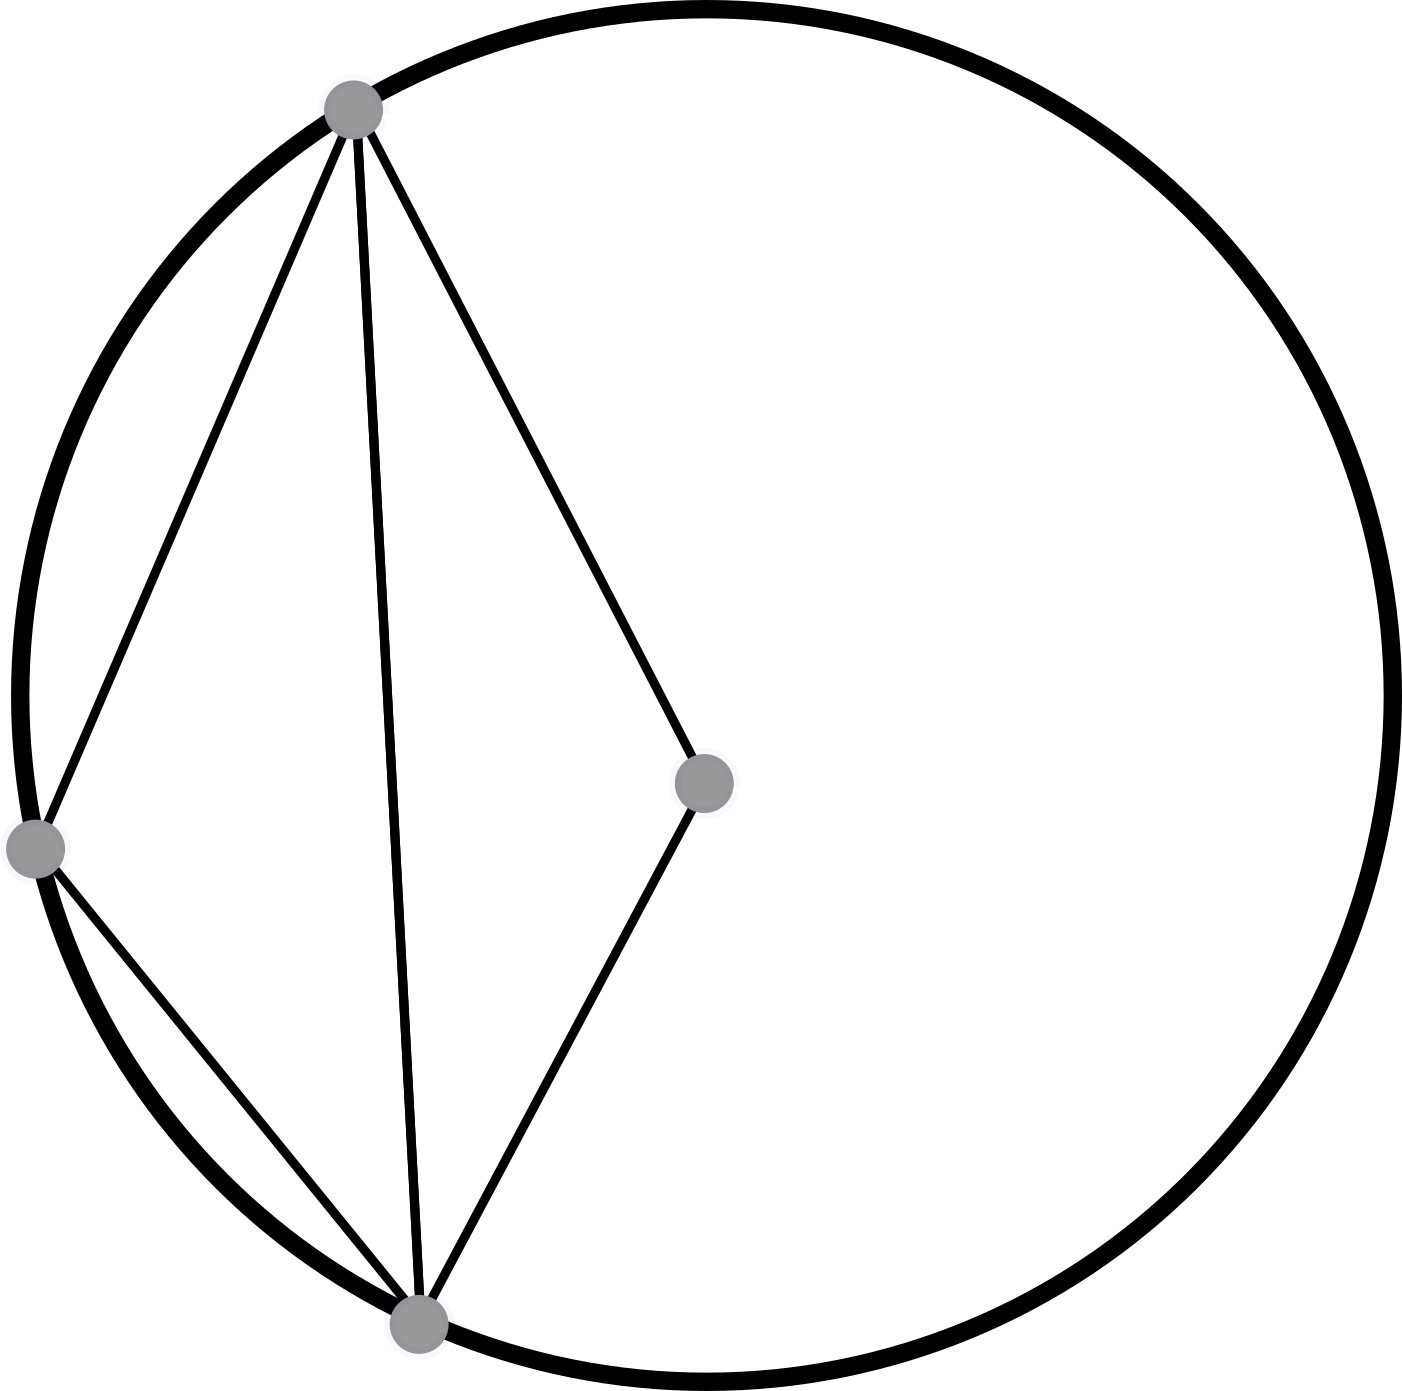
\includegraphics[scale=0.8]{dessin2}
\end{figure}
\end{frame}

\subsection{CC Systems}

\begin{frame}
 
 We tried to stay at the most abstract level possible to only do combinatorial proofs: CC Systems seemed a good way to express the clockwise ordering of points.
 
 \begin{definition}<2->
  CC (counter-clockwise) Systems are a ternary relation used to show the counter-clockwise ordering of triples of points $pqr$ in general position in the plane.
 \end{definition}
 

\end{frame}

\begin{frame}

 A CC system has to follow five axioms.
\begin{enumerate}
\item<1-> Cyclicity: $abc \rightarrow bca$.
\item<2-> Antisymmetry: $abc\rightarrow \neg bac$.
\item<3-> Nondegeneracy: $abc \vee bac$ since $a$ $b$ and $c$ can't be aligned.
\item<4-> Interiority: $abd \rightarrow bcd \rightarrow adc \rightarrow abc$.
\item<5-> Transitivity: $ abc \rightarrow abd \rightarrow abq \rightarrow cbd \rightarrow dbq \rightarrow cbq $.
\end{enumerate}

\begin{overprint}
\onslide<4>
\begin{figure}
  \centering
  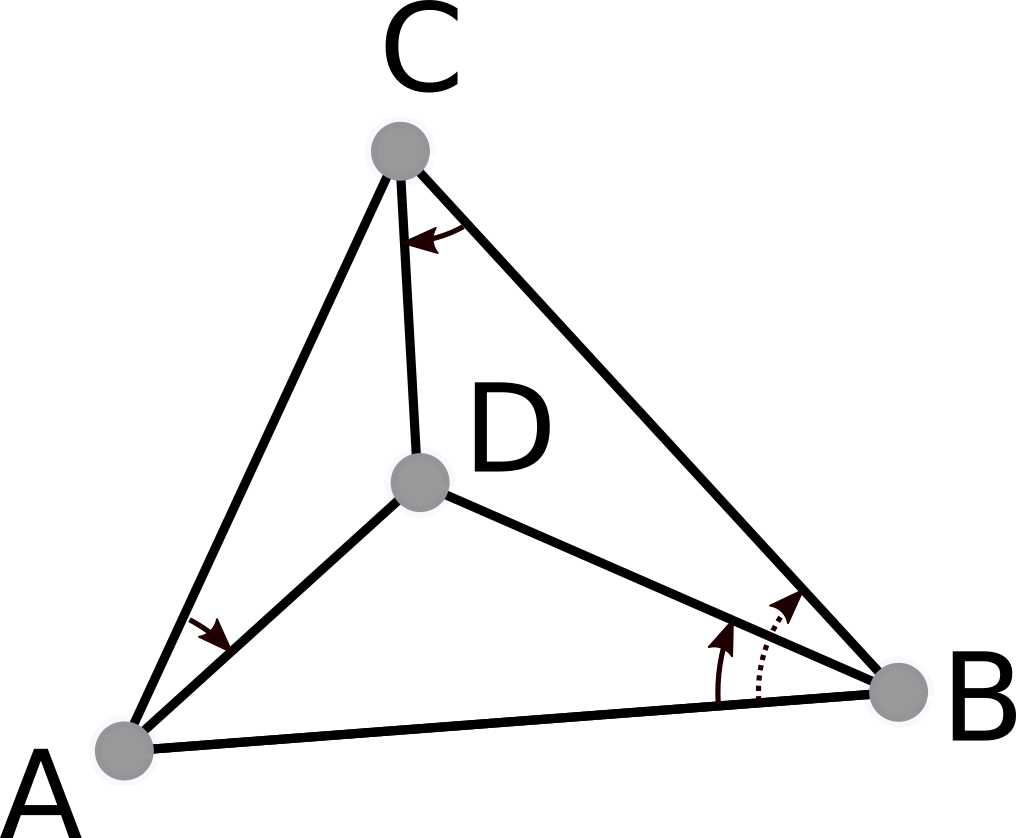
\includegraphics[scale=1.5]{Axiom4}
  \caption{Knuth's $4^{th}$ axiom.}
\end{figure}

\onslide<5>
\begin{figure}
  \centering
  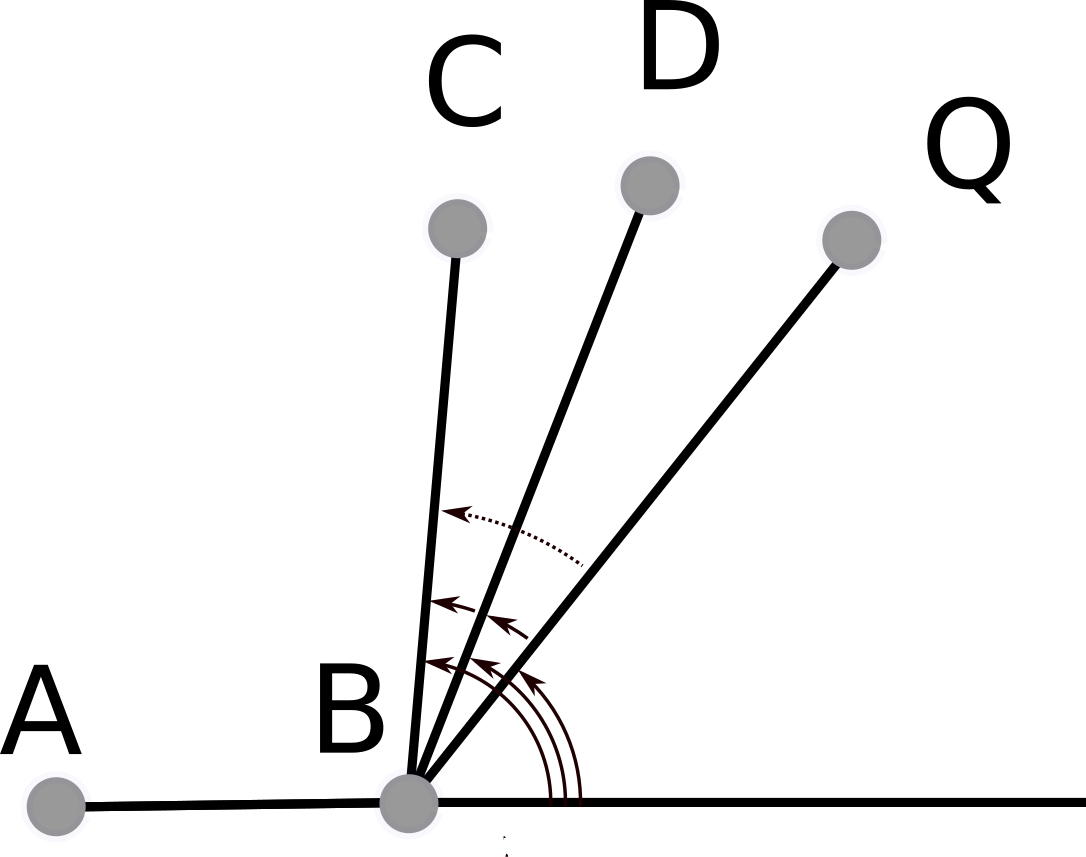
\includegraphics[scale=1.4 ]{Axiom5}
  \caption{Knuth's $5^{th}$ axiom.}
\end{figure}
\end{overprint}

\end{frame}


\section{The Algorithm}

\begin{frame}
Given an existing triangulation and a point, the algorithm consists in:
\begin{enumerate}
\item<1-> adding the point to the existing triangulation;
\item<2-> flipping the illegal edges to obtain a Delaunay triangulation.
\end{enumerate}
\end{frame}


\subsection{Adding Points}

\begin{frame}{Adding Points}
Three cases:

\begin{enumerate}
\item<1-> the new point is in the interior of a triangle of the triangulation;
\item<2-> the new point is on an edge of a triangle of the triangulation;
\item<3-> the new point is not in the convex hull of the existing triangulation.
\end{enumerate}

\begin{overprint}
  \onslide<1>
  \begin{figure}
\centering
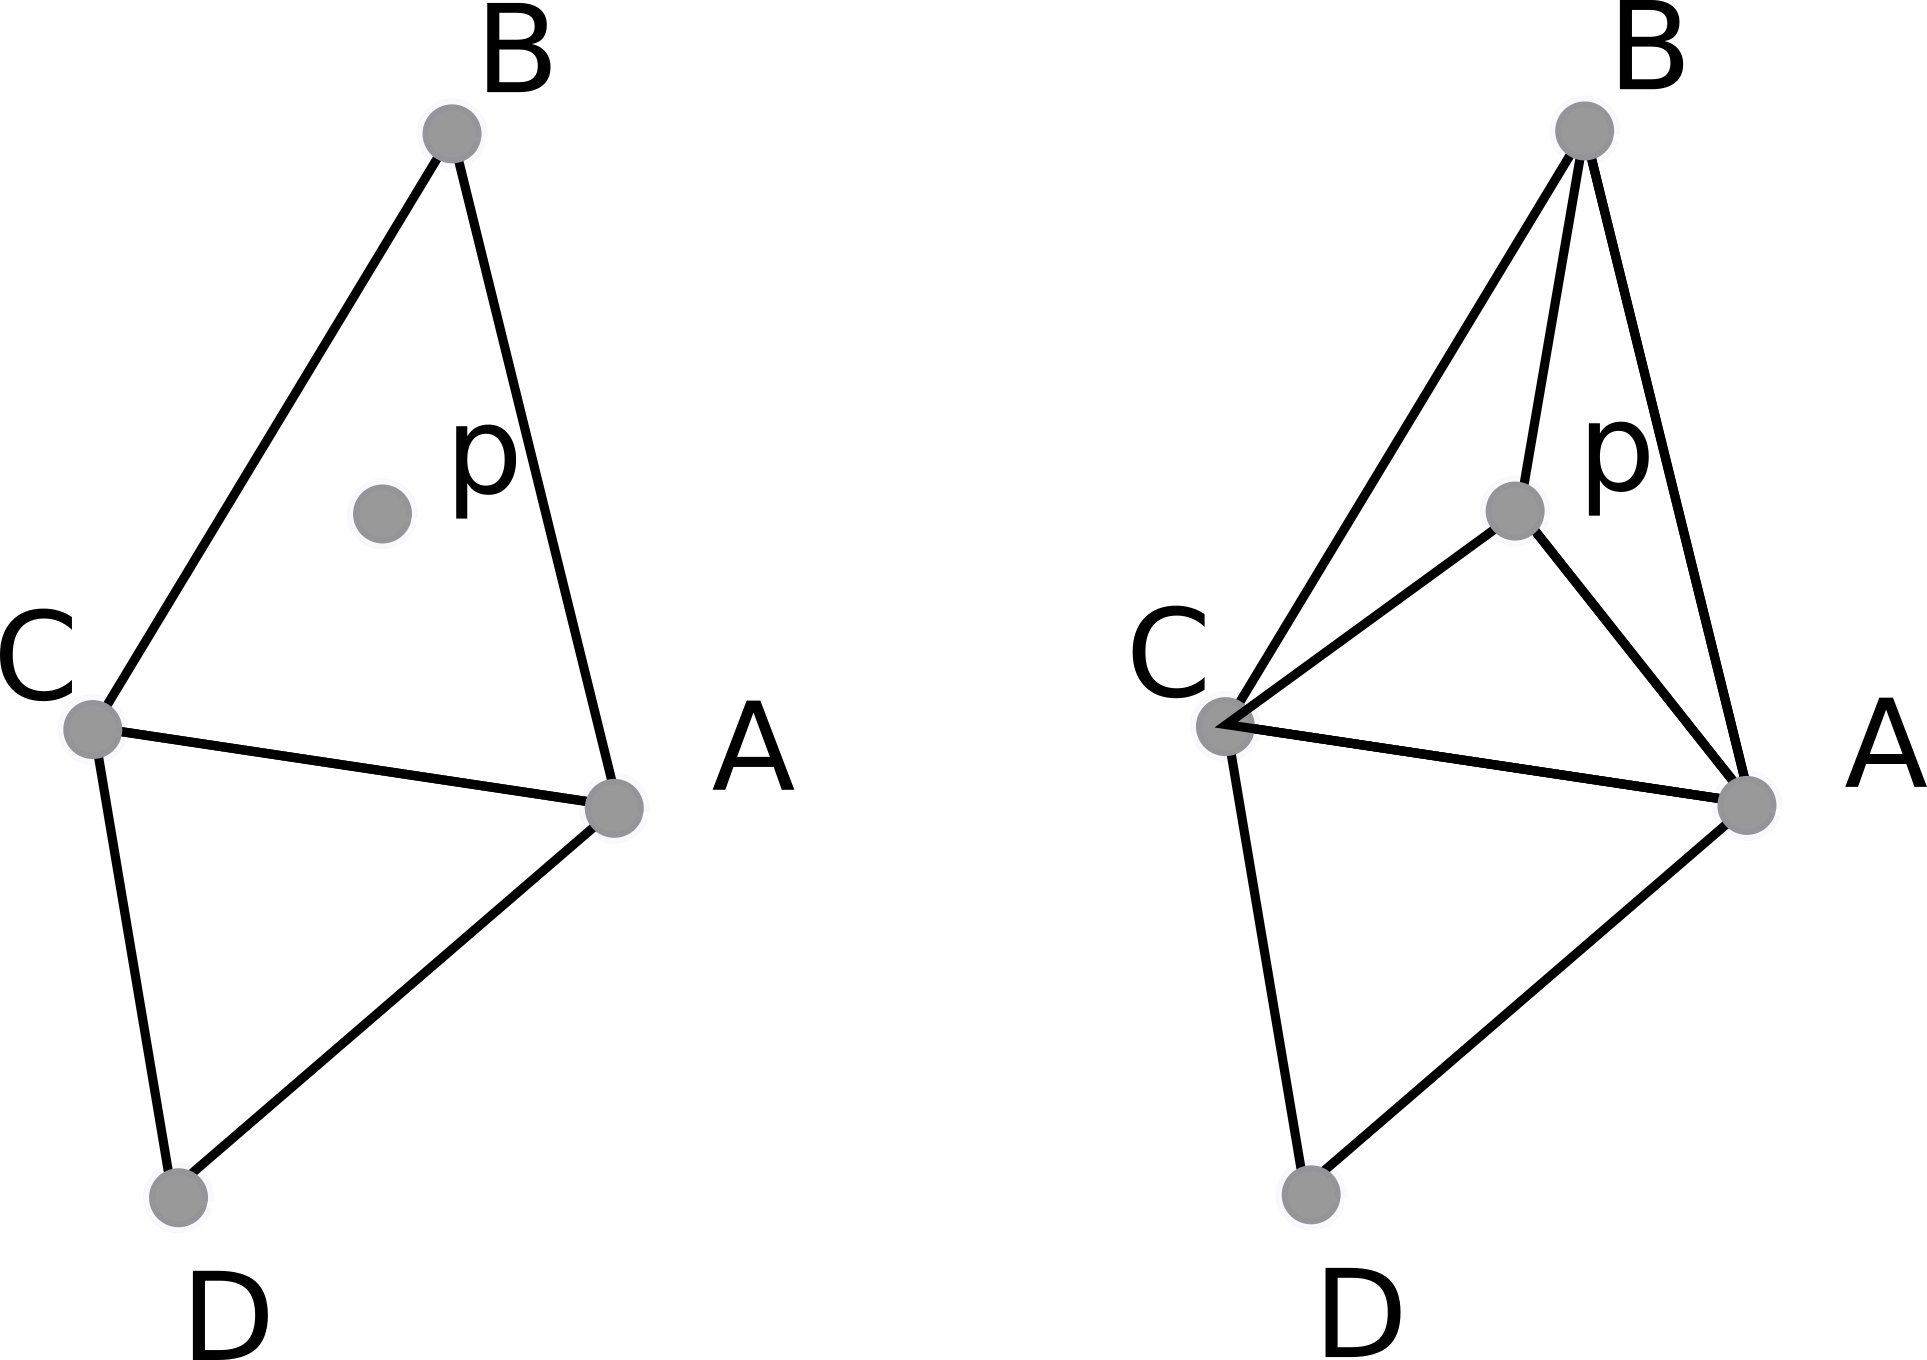
\includegraphics[scale=0.8]{adding}
\caption{Adding a point to a triangulation.}
\end{figure}
  \onslide<2>
  
  \begin{figure}
\centering
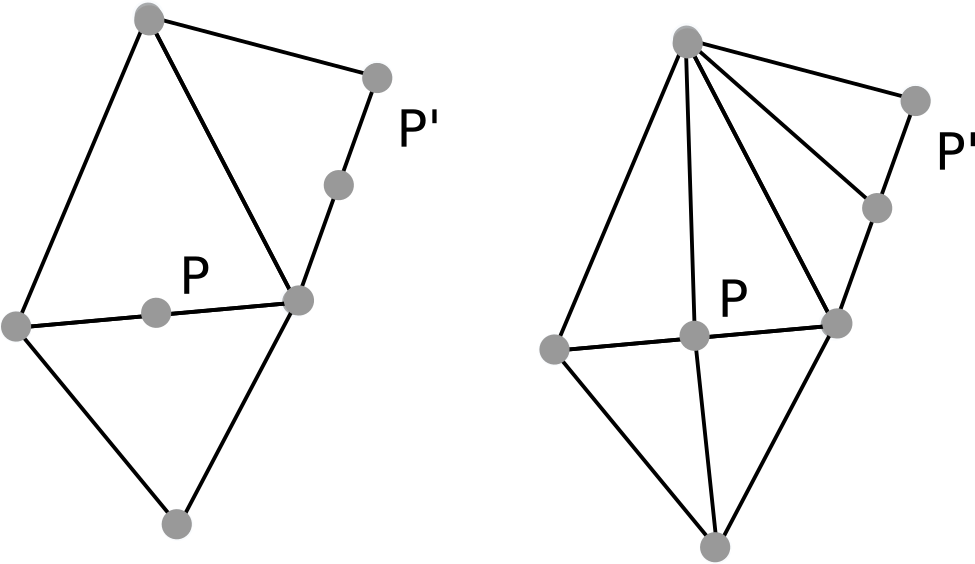
\includegraphics[scale=0.8]{adding2}
\caption{Adding a point to a triangulation.}
\end{figure}
  
  \onslide<3>
  
  \begin{figure}
\centering
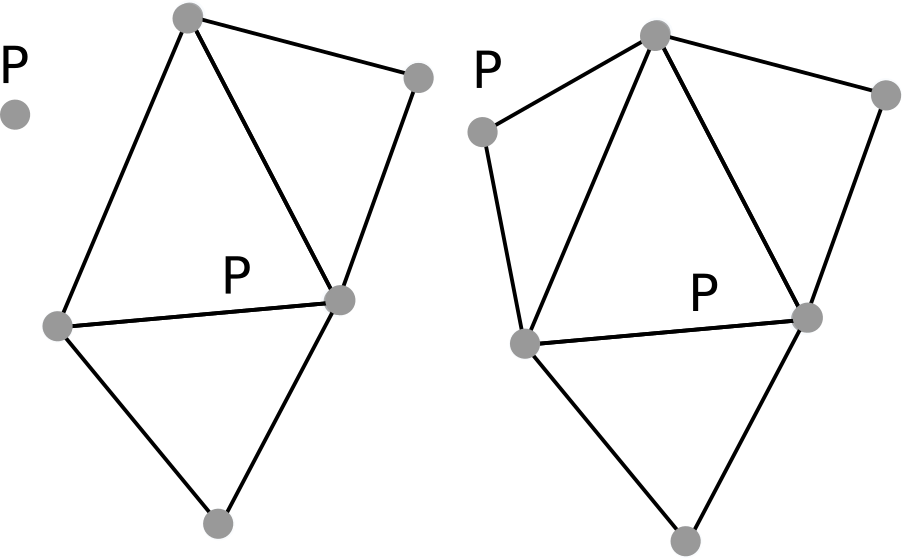
\includegraphics[scale=0.8]{adding3}
\caption{Adding a point to a triangulation.}
\end{figure}

\end{overprint}


\end{frame}


\subsection{Flipping Edges}
\begin{frame}{Transforming a triangulation into a Delaunay triangulation}

Obtain a Delaunay triangulation by repeating the same step: for each pair of triangles that does not meet the Delaunay condition, flip the common edge of the two triangles.

\begin{figure}
\centering

\includegraphics[scale=1]{dessin1}
\caption{\label{DelaunayTriangulation} From non-Delaunay triangulation to Delaunay triangulation.}
\end{figure}
 
\end{frame}


\section{The Formalisation}


\subsection{Functions and Geometrical Predicates}

\begin{frame}{What we require}
 
 We require in any instantiation of the formalisation:
 \begin{itemize}
  \item some functions ({\tt vertices\_to\_triangle}, ...),
  \item some Geometrical predicates.
 \end{itemize}
Geometrical predicates include:
\begin{itemize}
 \item<2-> {\tt is\_left\_of},
 \item<3-> {\tt is\_left\_or\_on\_line},
 \item<4-> {\tt in\_circle},
  \item<5-> {\tt is\_on\_line}.
\end{itemize}
\end{frame}
\begin{frame}{\tt in\_triangle}
From those predicates, we define what it is to be in a triangle:
{\small \begin{tabular}{ll}
       {\tt in\_triangle t p = }& {\tt is\_left\_of (vertex1 t) (vertex2 t) p} $\wedge$\\
        &{\tt is\_left\_of p (vertex2 t) (vertex3 t)} $\wedge$\\
  & {\tt is\_left\_of (vertex1 t) p (vertex3 t)}
      \end{tabular}}
      
       \begin{figure}
  \centering
  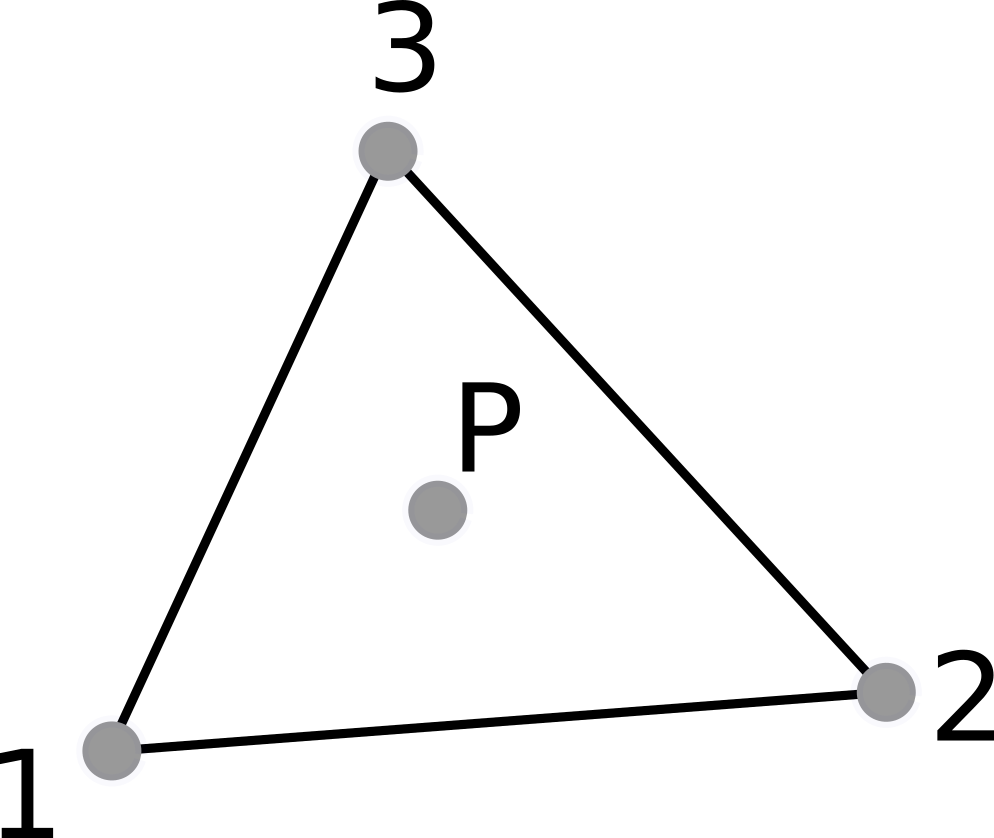
\includegraphics[scale=1]{intriangle}
  \caption{Here, $P$ is in $123$.}
\end{figure}
\end{frame}
\begin{frame}{\tt oriented\_surface}
We derive three of those predicates from a function, {\tt oriented\_surface}:
{\small   \begin{itemize}
\item<2-> {\tt is\_left\_of a b c = oriented\_surface a b c > 0};
  \item<3-> {\tt is\_left\_or\_on\_line a b c = oriented\_surface a b c $\geq$ 0};
  \item<4> {\tt is\_on\_line a b c = oriented\_surface a b c = 0}.
 \end{itemize} }

  \begin{overprint}
   \onslide<4>
  \begin{figure}
  \centering
  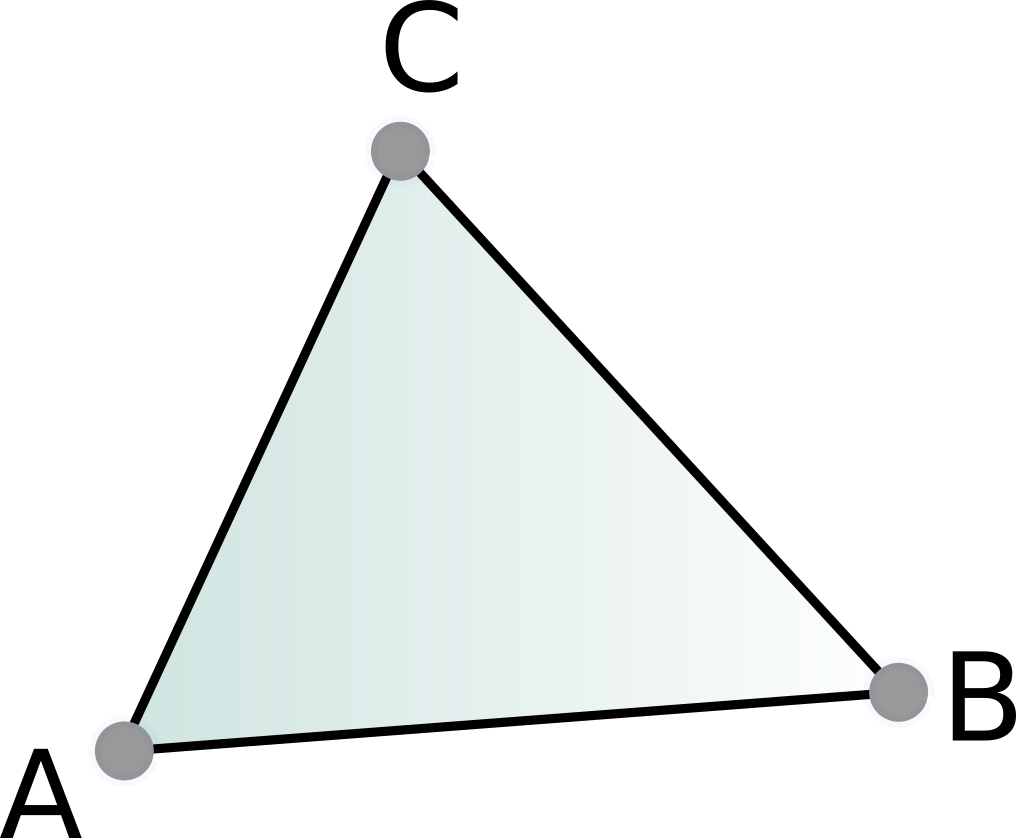
\includegraphics[scale=1]{Surface}
  \caption{\label{surface} Here, ABC has a positive oriented surface whereas ACB has a negative oriented surface.}
\end{figure}
  \end{overprint}

\end{frame}


\subsection{Hypotheses}

\begin{frame}{}
 We put assumptions on these functions and predicates. For instance:
 \begin{itemize}
  \item<1-> the oriented surface of a segment should be 0;
  \item<2-> the oriented surface of cab is the same as abc;
  \item<3-> the vertices of the triangle created by {\tt vertices\_to\_triangle a b c} should be  {\tt a} {\tt b} and {\tt c}.
 \end{itemize}

\end{frame}


\subsection{Geometrical Properties}

\begin{frame}
 A triangulation {\tt Tr} on a data set {\tt D} is a finite set of triangles with points of {\tt D} as vertices which satisfies the following properties:
\begin{enumerate}
\item<2-> {\tt covers\_hull}  \tikzmark{start}
\item<2-> {\tt covers\_vertices} \tikzmark{end}
\item<3-> {\tt no\_cover\_intersection}\tikzmark{start2}
\item<3-> {\tt no\_point\_on\_segment \hspace{0.2 cm}}\tikzmark{end2}
\item<4-> {\tt triangle\_3\_vertices}\tikzmark{start3}
\item<4-> {\tt triangle\_nempty}
\item<4-> {\tt oriented\_triangle\_triangulation} \tikzmark{end3}
\end{enumerate}
\begin{uncoverenv}<2->
\begin{tikzpicture}[remember picture,overlay]
\draw[decorate,decoration={brace,raise=12pt}]
  ([yshift=2ex]{{pic cs:end}|-{pic cs:start}}) --
    node[xshift=15pt,anchor=west] {Tiling of the convex hull.} 
  ([yshift=-0.5ex]pic cs:end);
\end{tikzpicture}
\end{uncoverenv}

\begin{uncoverenv}<3->

\begin{tikzpicture}[remember picture,overlay]
\draw[decorate,decoration={brace,raise=12pt}]
  ([yshift=2ex]{{pic cs:end2}|-{pic cs:start2}}) --
    node[xshift=15pt,anchor=west] {Intersection of simplices.} 
  ([yshift=-0.5ex]pic cs:end2);
\end{tikzpicture}
\end{uncoverenv}

\begin{uncoverenv}<4->
\begin{tikzpicture}[remember picture,overlay]
\draw[decorate,decoration={brace,raise=12pt}]
  ([yshift=2ex]{{pic cs:end3}|-{pic cs:start3}}) --
    node[xshift=15pt,anchor=west] {No degenerate triangles.} 
  ([yshift=-0.5ex]pic cs:end3);
\end{tikzpicture}
\end{uncoverenv}

\end{frame}


\section{Operations and Proofs}

\begin{frame}{Operations}
The two operations written:
 \begin{itemize}
  \item<1-> Given a triangle $t = ABC$, a point $p$ which is an interior point of $t$, a triangulation $tr$, {\tt split\_triangle $tr$ $t$ $p$} returns $(tr \smallsetminus t) \cup \{ABp;pBC;ApC\}$
  \item<2-> Given $t1 = abc$ and $t2=acd$, {\tt flip\_edge $tr$ $t1$ $t2$ $a$ $b$ $c$ $d$} returns $(tr \smallsetminus t1 \smallsetminus t2) \cup \{abd;bcd\}$.
 \end{itemize}
\begin{overprint}
 \onslide<1>
 \begin{figure}
  \centering
  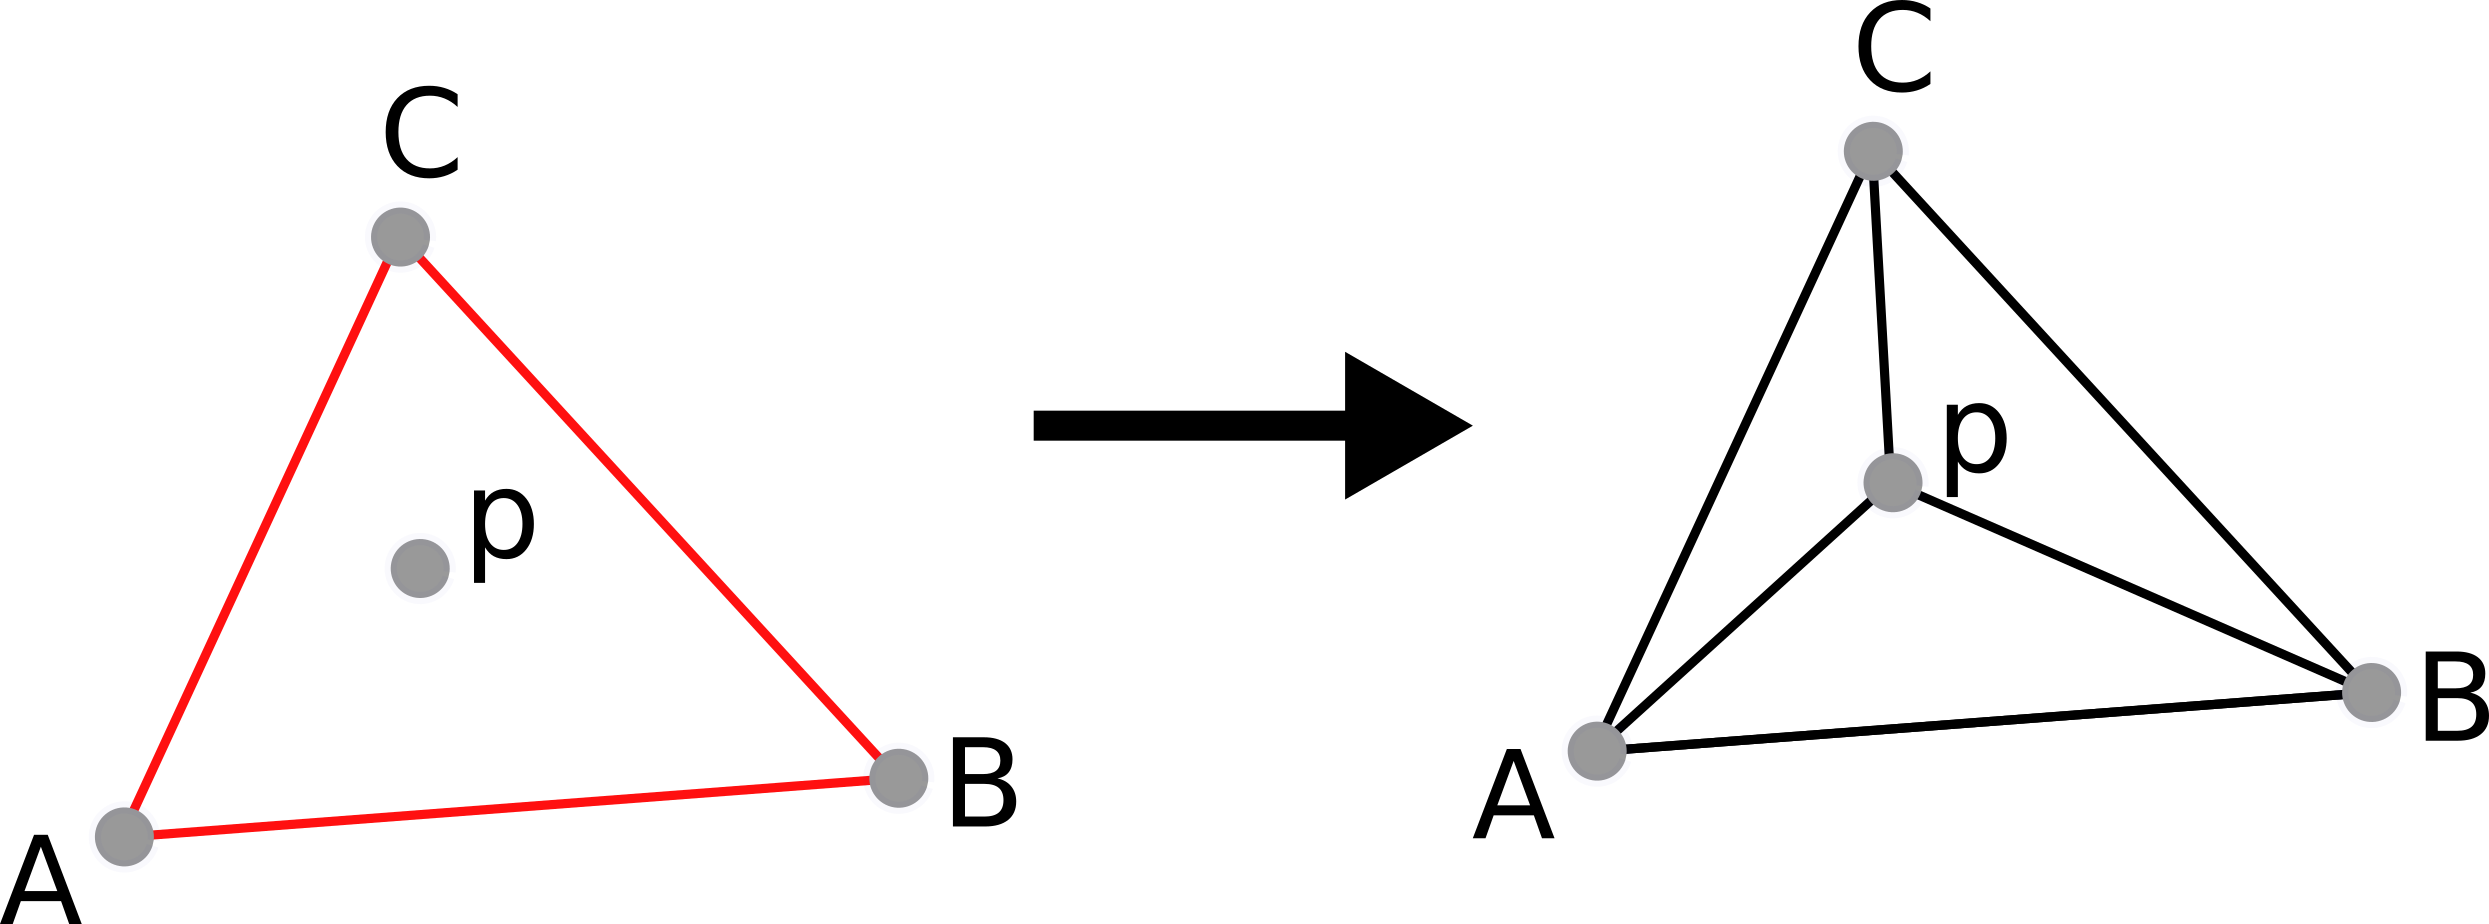
\includegraphics[scale=1.2]{split_triangle}
    \caption{{\tt split\_triangle}}
\end{figure}
 \onslide<2>
 \begin{figure}
  \centering
  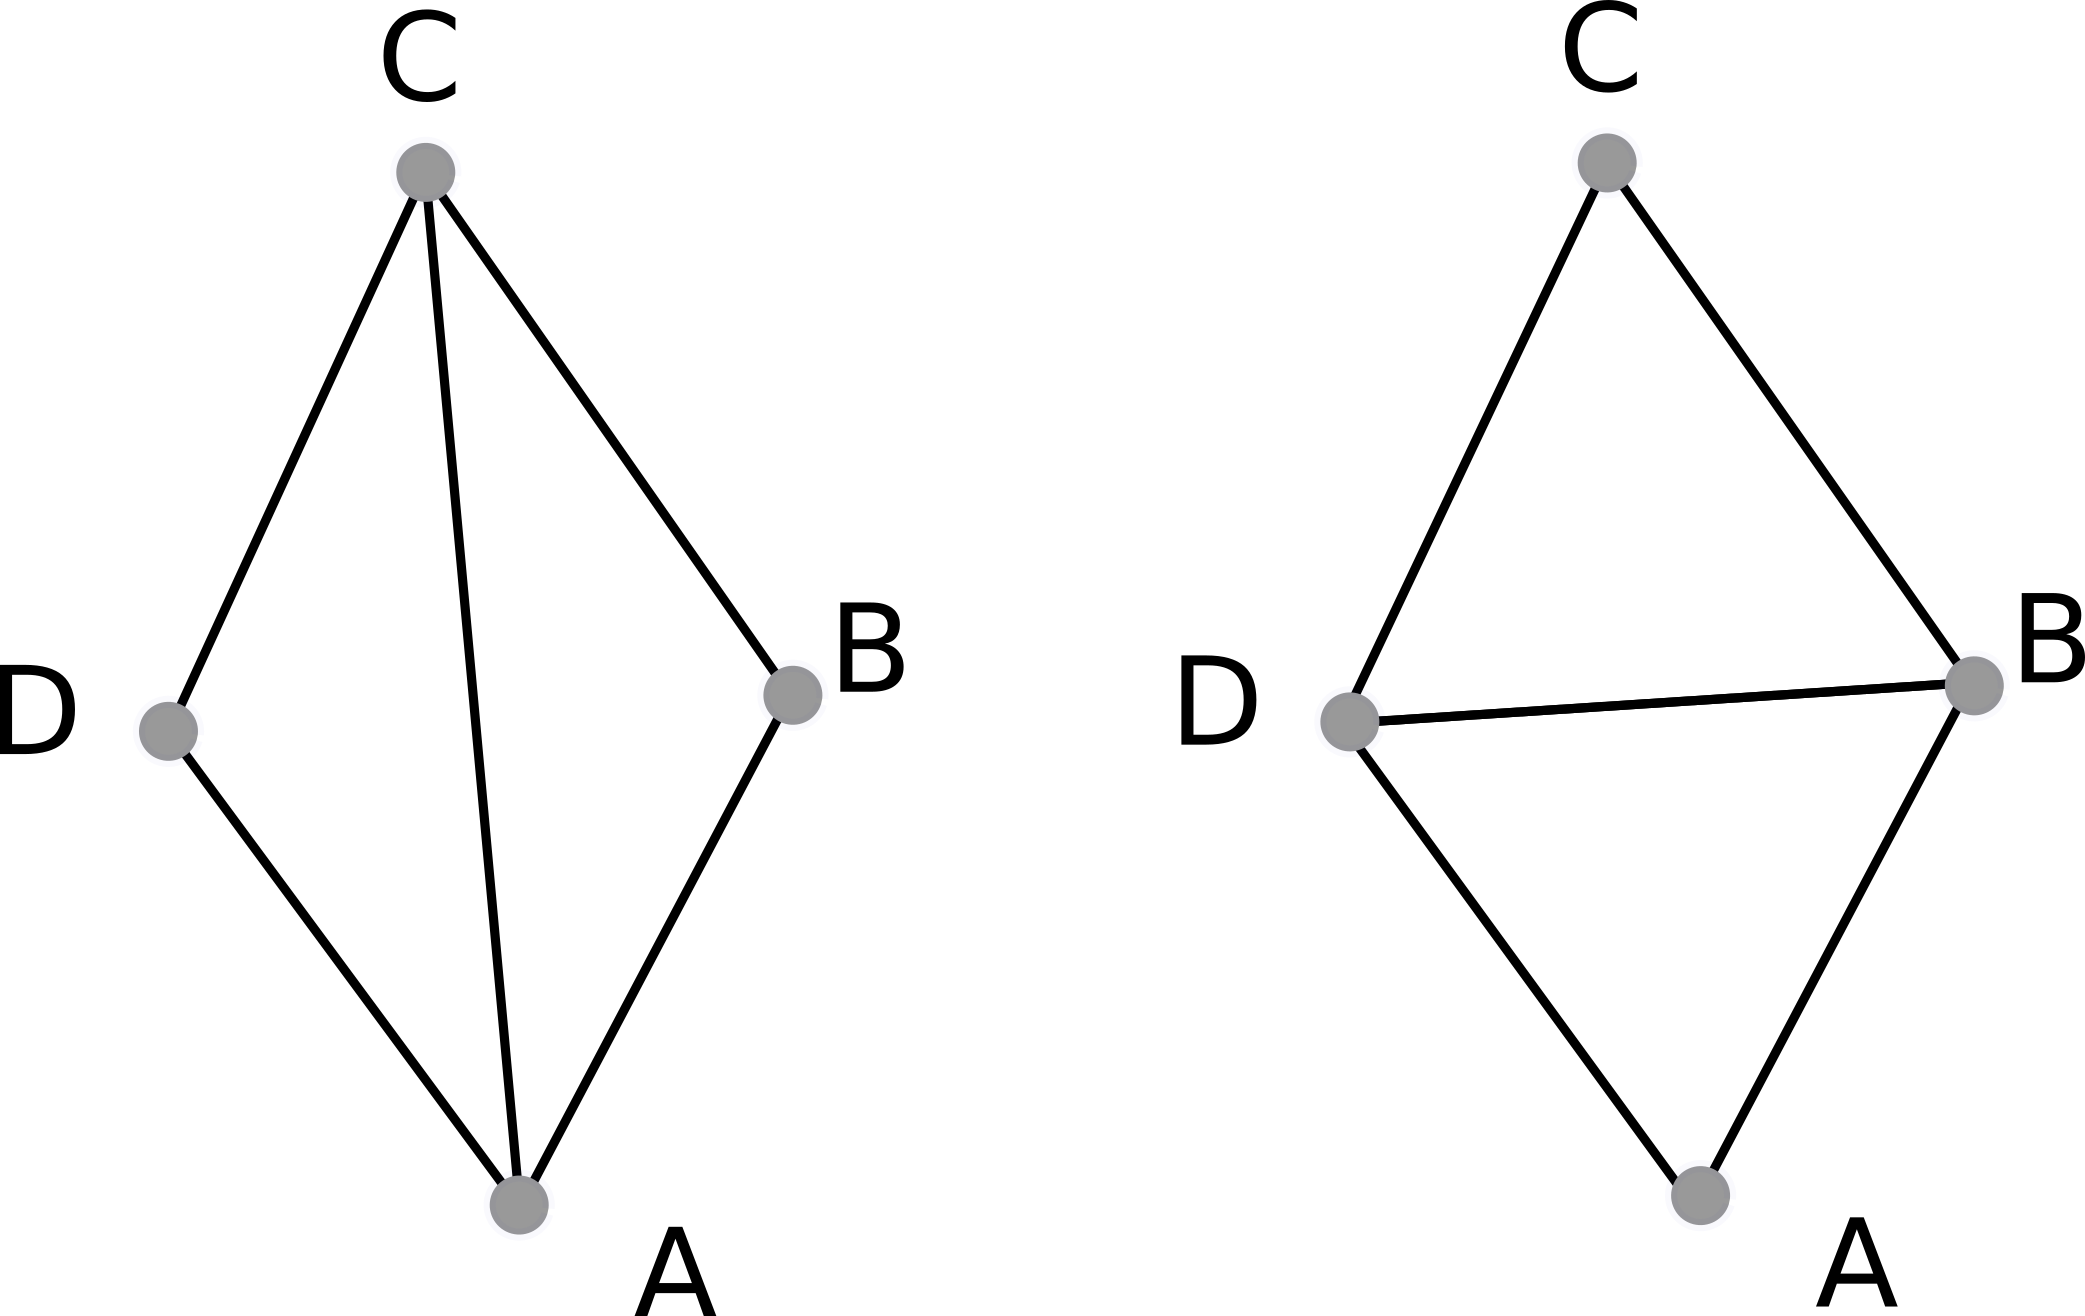
\includegraphics[scale=0.8]{flip_edge}
    \caption{\label{flip_edge} An edge-flipping step.}
\end{figure}

\end{overprint}

\end{frame}

\begin{frame}{Difficulties encountered}
Idea of the proofs: case-based reasonning, with some intermediary lemmas.

Some common difficulties:
\begin{itemize}
 \item<2-> Number of similar cases slowing down the proofs.
 \item<3-> Problems of symmetry ({\tt is\_left\_of a b c} vs {\tt is\_left\_of c a b}): a first try with {\tt easygeo}.
\end{itemize}

\end{frame}


\section{Conclusion}
\begin{frame}
Work done:
\begin{itemize}
 \item Formalisation of the Delaunay triangulation
 \item Two steps of the algorithm, the proofs of their correctness, the proof of some relevant lemmas.
 \item An instantiation of the model
\end{itemize}

\begin{uncoverenv}<2>
What to do now ?
\begin{itemize}
 \item Finish the proofs.
 \item Find a better way to use the symmetry.
 \item Higher dimensions.
 \item Better algorithms.
\end{itemize}
\end{uncoverenv}
\end{frame}


\begin{frame}
\begin{centering}
 Thank you for your attention !
\end{centering}

\end{frame}




\end{document}
